\documentclass[aspectratio=169,11pt]{beamer}

% Shared style (ib-tutorials.sty at the repo root).
\makeatletter\def\input@path{{./}{../}}\makeatother
\usepackage{ib-tutorials}

\usepackage[utf8]{inputenc}
\usepackage{amsmath,amssymb}
\usepackage{booktabs}
\usepackage{array}
\newcolumntype{L}[1]{>{\raggedright\arraybackslash}p{#1}}
\usepackage{graphicx}
\graphicspath{{../pictures/4-ibfe/}{pictures/4-ibfe/}}
\usepackage{xcolor}
\usepackage{listings}
\usepackage{tikz}
\usetikzlibrary{arrows.meta,positioning,shapes.geometric,fit,calc,decorations.pathmorphing}
\usepackage{hyperref}

\newcommand{\sourcecredit}[1]{\vfill\begin{flushright}\tiny\textcolor{DarkGray}{#1}\end{flushright}}

\lstset{
  basicstyle=\ttfamily\scriptsize\color{BlackGray},
  keywordstyle=\color{NavyBlue}\bfseries,
  commentstyle=\color{DarkGray}\itshape,
  stringstyle=\color{OliveGreen},
  showstringspaces=false,
  columns=fullflexible,
  keepspaces=true,
  breaklines=true,
  breakindent=1em,
  frame=single,
  framerule=0.4pt,
  rulecolor=\color{LightGray},
  backgroundcolor=\color{LightGray!30},
  xleftmargin=0.25em,
  xrightmargin=0.25em
}
\lstdefinestyle{shell}{morecomment=[l]{\#}}
\lstdefinestyle{input}{morecomment=[l]{//}}
\lstdefinestyle{matlab}{morecomment=[l]{\%}}
\lstdefinestyle{python}{morecomment=[l]{\#}}
\lstdefinestyle{data}{}
\lstdefinestyle{tiny}{basicstyle=\ttfamily\tiny\color{BlackGray}}
\lstdefinestyle{inputtiny}{morecomment=[l]{//},basicstyle=\ttfamily\tiny\color{BlackGray}}
\lstdefinestyle{cpp}{language=C++,morecomment=[l]{//}}
\lstdefinestyle{cpptiny}{language=C++,morecomment=[l]{//},basicstyle=\ttfamily\tiny\color{BlackGray}}

\title[Fibre tension and active stress]{Fibre tension and active stress}
\subtitle{An active stress along fibres as a third registered stress: the formula and what its $T$ means, the course's three fibre-tension examples run (IBFE/06), the homework and its two solutions, and the jellyfish template}
\author[Miller]{Laura A. Miller}
\institute[UArizona]{Department of Mathematics, University of Arizona}
\date{Using IB Software \textbullet\ Part IV \textbullet\ Chapter 20}

\begin{document}

% 1
\begin{frame}[plain]
\maketutorialtitlepanel{%
\begin{tikzpicture}[scale=0.84]
  % a plate with fibres and a travelling pulse of tension
  \draw[BlackGray,thick] (0.3,1.2) rectangle (3.9,1.5);
  \foreach \y in {1.27,1.35,1.43} \draw[NavyBlue,thin] (0.35,\y) -- (3.85,\y);
  \fill[RubineRed,opacity=0.35] (2.1,1.2) rectangle (2.7,1.5);
  \draw[-{Stealth[length=1.6mm]},RubineRed,thick] (1.75,1.35) -- (2.05,1.35);
  \draw[-{Stealth[length=1.6mm]},RubineRed,thick] (3.05,1.35) -- (2.75,1.35);
  \draw[-{Stealth[length=1.6mm]},DarkGray] (2.4,1.7) -- (3.0,1.7);
  \node[font=\tiny,text=DarkGray] at (2.7,1.9) {$x_c = t - \tfrac12$};
  \node[font=\tiny,text=NavyBlue] at (0.9,0.95) {$\mathbf{f}_0 = (1, 0)$};
  \node[font=\footnotesize,text=OliveGreen] at (2.1,0.55) {$\mathbb{P}_a = J\,T(\mathbf{s},t)\,\mathbb{F}\,\mathbf{f}_0\otimes\mathbf{f}_0$};
  \node[font=\tiny,text=DarkGray] at (2.1,0.15) {true tension $T\lambda^2$, $\lambda = |\mathbb{F}\mathbf{f}_0|$};
\end{tikzpicture}}
\end{frame}

% 2
\begin{frame}{Learning goals}
\label{fr:goals}
\footnotesize By the end of this chapter you should be able to:
\begin{enumerate}
  \item add an active stress along a fibre direction to the passive material law, as a third registered stress function, and say in which frame its tension $T$ lives (the reference one) and what the true tension in the deformed body is ($T\lambda^2$);
  \item write $T(\mathbf{s}, t)$ for a muscle that contracts on a schedule, a pulse that travels along the body, and a pulse confined to one side, and say what each does to a free plate: the course's three examples, run as IBFE/06;
  \item write the course homework's travelling sine wave with a tension that never goes negative, and the out-of-phase version, and say why the 2017 solution's phase shift is $206^\circ$ rather than $180^\circ$;
  \item give the fibre direction as a function of reference position (circumferential fibres of a jellyfish bell) and know where the two conventions, mapped fibre and unit fibre, differ, including in a 2014 example that used both at once;
  \item find the oblate jellyfish template in the research-code collection and read its activation function;
  \item choose $T_{\max}$ against $\mu$ and read the plate's shortening and swimming from the output.
\end{enumerate}
\begin{punchbox}
\footnotesize Chapter 19 gave the passive stress; this chapter adds the muscle. The theory repository's 4.3 (``Passive and active stress'', ``Fiber-oriented active stress'', ``Jellyfish circumferential reference fibers'', ``Jellyfish activation field'') has the derivation; here is the code and what it did.
\end{punchbox}
\end{frame}

% 3
\begin{frame}{Where this chapter comes from}
\label{fr:sources}
\scriptsize
\begin{itemize}
  \item \al{Alex Hoover, ``4-IBFE Tutorial: Fiber Tension'' (2014, edited 2020; 12 slides, 6 renders):} the idea, three examples on a horizontal beam (static, moving, alternating) with their \code{active\_stress\_function}s, a homework, and links to two solution folders. The 2020 lab deck's slides 15--23 are the same text with the nine-argument signature; its slide 21 kept the old seven-argument one.
  \item \al{The example folders:} generation 1 (2014, \code{IBAMR\_IBFE\_Module\_3803\_Examples}: \code{FiberStress2D}, \code{MovingFiberStress2D}, \code{AltMovingFiberStress2D}, \code{OscillatingMuscleFiber2D}), generation 3 (2017, \code{IBFE\_Module\_2016-11\_Examples}: the first three ported, plus the homework solutions \code{MovingSinusoidalFiberStress2D} and \code{MovingAltSinusoidalFiberStress2D}, with their output). Example IBFE/06 is the first three in one program; the solutions and the oscillating-muscle code are quoted on slides \ref{fr:homework2} and \ref{fr:oscillating}.
  \item \al{The theory repository, chapter 4.3, section ``Active stress and biological examples'':} the passive--active split, the mapped-fibre convention and its Cauchy counterpart, the jellyfish's circumferential fibres and activation field, after Hoover, Griffith and Miller (2017).
  \item \al{The oblate jellyfish template} (\code{IBAMR-Research-Codes/Medusa/oblate\_jellyfish\_template\_uniform}, 2022 copy): a 3D bell with hexahedral mesh, the activation of that paper; a pointer, slide \ref{fr:jellyfish}.
  \item \al{New here:} the runs of the three modes with measured lengths, bends and swimming speed (IBFE/06's README); what $T$ means, with the Cauchy and second Piola--Kirchhoff forms; the convention clash inside the 2014 oscillating-muscle code; the homework solutions' formulas checked ($+\pi/2$ inside the argument); the stiffer-plate comparison; the active quadrature order.
\end{itemize}
\end{frame}

% 4
\begin{frame}{The idea}
\label{fr:idea}
\footnotesize
\begin{columns}[T]
\column{0.52\textwidth}
``Apply an active tension that plays the role of muscle. This tension acts in addition to the innate passive elastic tension of the structure due to the material model'' (2014).
\begin{itemize}
  \item Muscle shortens along its fibres. In the stress language of chapter 19 that is an \emph{added} stress $\mathbb{P}_a$ that pulls along a direction $\mathbf{f}_0$ fixed in the reference body: $\mathbb{P} = \mathbb{P}_{\mathrm{passive}} + \mathbb{P}_a$.
  \item It is not a body force: it acts between neighbouring material points, like the passive stress, and is integrated by parts the same way (chapter 19, slide 5). The theory repository: ``once expressed as PK1 stress, passive and active contributions use the same FE assembly and fluid-coupling operators.''
  \item ``This is a lot easier than in the fiber version of IBAMR'' (chapter 9b's springs with changing rest lengths): $T$ can be any function of the reference position and time.
\end{itemize}
\column{0.46\textwidth}
\begin{itemize}
  \item Three ingredients: a fibre direction $\mathbf{f}_0(\mathbf{s})$ (a unit vector in the reference configuration), a tension magnitude $T(\mathbf{s}, t) \ge 0$, and the rule that turns them into $\mathbb{P}_a$ (next slide).
  \item Registered like any stress: a third \code{PK1StressFcnData}, with its own quadrature order; ``stress components are additive''.
  \item The passive law stays: without it the contracted body would not spring back. $T$ against $\mu$ sets how far it shortens (slide \ref{fr:mu40}).
\end{itemize}
\begin{punchbox}
\footnotesize Where chapter 9a's target points \emph{tell} the body where to be, an active stress \emph{pushes} it: what happens next is decided by the material and the fluid.
\end{punchbox}
\end{columns}
\end{frame}

% 5
\begin{frame}{The formula, and what $T$ means}
\label{fr:formula}
\footnotesize
\begin{columns}[T]
\column{0.5\textwidth}
With $\mathbf{f}_0$ the reference fibre direction (unit), $\mathbb{F}$ the deformation gradient and $J = \det\mathbb{F}$:
\[ \mathbb{P}_a = J\,T\,\mathbb{F}\,(\mathbf{f}_0\otimes\mathbf{f}_0),\qquad (\mathbf{f}_0\otimes\mathbf{f}_0)_{ij} = f_{0i}f_{0j}. \]
\begin{itemize}
  \item In the deformed body the fibre has become $\mathbf{a} = \mathbb{F}\mathbf{f}_0$, of length $\lambda = |\mathbf{a}|$, pointing along $\mathbf{f} = \mathbf{a}/\lambda$. The Cauchy stress of the active part is $\boldsymbol{\sigma}_a = J^{-1}\mathbb{P}_a\mathbb{F}^T = T\,\mathbf{a}\otimes\mathbf{a} = T\lambda^2\,\mathbf{f}\otimes\mathbf{f}$: \al{the true tension is $T\lambda^2$}, not $T$.
  \item The second Piola--Kirchhoff stress is $\mathbb{S} = \mathbb{F}^{-1}\mathbb{P}_a = J\,T\,\mathbf{f}_0\otimes\mathbf{f}_0$: $T$ lives entirely in the reference configuration.
  \item The two agree only while the fibres are unstretched. When the plate contracts, $\lambda < 1$ and the true tension is smaller: at the STATIC run's shortest, $\lambda \approx 0.68$ and $20\times0.68^2 \approx 9$.
\end{itemize}
\column{0.48\textwidth}
\begin{itemize}
  \item This is the theory repository's \emph{mapped-fibre convention}, $\boldsymbol{\sigma}_a = T\,\mathbf{a}\otimes\mathbf{a}$. The other common one, the \emph{unit-fibre} law $\boldsymbol{\sigma}_a = \widehat{T}\,\mathbf{f}\otimes\mathbf{f}$, pulls back to $\mathbb{P}_a = J\,\widehat{T}\lambda^{-2}\,\mathbb{F}\,\mathbf{f}_0\otimes\mathbf{f}_0$: the same shape with a different power of $\lambda$. ``The scalar $T$ must be calibrated for the convention used''; a $T_{\max}$ from one paper cannot be moved to the other law unchanged.
  \item The sign of $\mathbf{f}_0$ does not matter: only $\mathbf{f}_0\otimes\mathbf{f}_0$ enters. The course files used $(-1, 0)$; the example uses $(1, 0)$ and gives the same stress to the last digit.
  \item $T < 0$ would be a push along the fibres; muscle does not push, and a pushed slender body buckles. Keep $T \ge 0$ (slide \ref{fr:homework}).
\end{itemize}
\end{columns}
\end{frame}

% 6
\begin{frame}[fragile]{The code (IBFE/06): the tension and the stress}
\label{fr:code}
\begin{lstlisting}[style=cpptiny]
// TENSION_STATIC / _MOVING / _ALTERNATING and PULSE_WIDTH come from the input
static double T_max = 20.0;
static double pulse_width = 0.1;
// fibres along the plate, in the reference configuration
static const VectorValue<double> f_0(1.0, 0.0);

double active_tension(const libMesh::Point& s, const double time)
{
    const double t_cycle = time - std::floor(time);   // time within the current 1 s cycle
    switch (fiber_mode)
    {
    case FiberMode::STATIC:                           // the whole plate, first half of each cycle
        return (t_cycle < 0.5) ? T_max : 0.0;
    case FiberMode::MOVING:
    case FiberMode::ALTERNATING:
    {   // a Gaussian pulse whose centre moves from x = -0.5 to 0.5 each cycle;
        // with ALTERNATING only the bottom half (s(1) < 0) is active
        if (fiber_mode == FiberMode::ALTERNATING && s(1) >= 0.0) return 0.0;
        const double x_c = t_cycle - 0.5;
        return T_max * std::exp(-(s(0) - x_c) * (s(0) - x_c) / (pulse_width * pulse_width));
    }
    }
    return 0.0;
}
\end{lstlisting}
\end{frame}

% 6b
\begin{frame}[fragile]{The code (2): the stress function}
\label{fr:code2}
\begin{lstlisting}[style=cpptiny]
void active_stress_function(TensorValue<double>& PP, const TensorValue<double>& FF,
                            const libMesh::Point& /*X*/, const libMesh::Point& s, Elem* const /*elem*/,
                            const std::vector<const std::vector<double>*>& /*var_data*/,
                            const std::vector<const std::vector<VectorValue<double> >*>& /*grad_var_data*/,
                            double time, void* /*ctx*/)
{
    const double T = active_tension(s, time);
    if (T == 0.0)
    {
        PP.zero();
        return;
    }
    TensorValue<double> f0_f0;
    outer_product(f0_f0, f_0, f_0);     // the tensor f_0 (x) f_0
    PP = FF.det() * T * FF * f0_f0;     // P_a = J T F (f_0 (x) f_0)
}
\end{lstlisting}
\footnotesize
\begin{itemize}
  \item The same nine arguments as every stress function (chapter 19, slide 9); only \code{FF}, \code{s} and \code{time} are used.
  \item \code{outer\_product(A, u, v)} fills $A_{ij} = u_iv_j$ (IBAMR's helper in \code{libmesh\_utilities.h}; the two-argument form returns the tensor). \code{FF.det()} is $J$; the product \code{FF * f0\_f0} is the matrix product $\mathbb{F}(\mathbf{f}_0\otimes\mathbf{f}_0)$.
  \item The early return for $T = 0$ saves the arithmetic on the half of each cycle (STATIC) or the part of the plate (ALTERNATING, the pulse's tails) where nothing is active: this function runs at every quadrature point every step.
\end{itemize}
\end{frame}

% 7
\begin{frame}[fragile]{The 2014 version, and its two small slips}
\label{fr:code2014}
\footnotesize
\begin{columns}[T]
\column{0.5\textwidth}
\code{FiberStress2D} (2014, slide 5; the 2016-11 port is the same):
\begin{lstlisting}[style=cpptiny]
static const VectorValue<double> f_0(-1,0);
void active_stress_function(
	TensorValue<double>& PP,
	const TensorValue<double>& FF,
	const libMesh::Point& X,
	const libMesh::Point& s,
	Elem* const /*elem*/,
	const vector<NumericVector<double>*>& /*system_data*/,
	double time,
	void* /*ctx*/)
{
	double T = 20; //provides a magnitude of tension
	if ((time - floor(time)) < 0.5) {    //if time is X - X.5, apply tension.
    	//const TensorValue<double> f_0(1,0);
    	double J = FF.det();
    	TensorValue<double> f_f;
    	outer_product(f_f, f_0, f_0);
    	PP = J * T * FF * f_f;
	}
	else {
    	PP.zero();    //set active tension to zero.
	}
}
\end{lstlisting}
\column{0.48\textwidth}
\begin{itemize}
  \item The commented-out second declaration, \code{const TensorValue<double> f\_0(1,0)}, has the wrong type: a fibre direction is a \code{VectorValue}. Uncommented it would shadow the real \code{f\_0} and \code{outer\_product} would not compile. It sat in every course copy from 2014 to 2024.
  \item The seven-argument signature (chapter 19, slide 9) is the 2014 one; the 2020 deck shows the nine-argument form on slides 17 and 19 and the old one on slide 21.
  \item \code{T = 20} inside the function; the example reads \code{TENSION\_STATIC} from the input.
  \item ``If time is $X - X.5$, where $X$ is an integer'': the first half of every second; \code{time - floor(time)} is the phase.
  \item The example's \code{active\_tension()} separates \emph{where and when} from \emph{how}: the three modes share one stress function.
\end{itemize}
\end{columns}
\end{frame}

% 8
\begin{frame}[fragile]{Registering the active stress: a third \code{PK1StressFcnData}}
\label{fr:register}
\footnotesize
The 2020 deck's slide 8 (and the example):
\begin{lstlisting}[style=cpptiny]
IBFEMethod::PK1StressFcnData active_stress_data(active_stress_function);
IBFEMethod::PK1StressFcnData PK1_dev_stress_data(PK1_dev_stress_function);
IBFEMethod::PK1StressFcnData PK1_dil_stress_data(PK1_dil_stress_function);
PK1_dev_stress_data.quad_order = Utility::string_to_enum<libMesh::Order>(input_db->getStringWithDefault("PK1_DEV_QUAD_ORDER", "THIRD"));
PK1_dil_stress_data.quad_order = Utility::string_to_enum<libMesh::Order>(input_db->getStringWithDefault("PK1_DIL_QUAD_ORDER", "FIRST"));
ib_method_ops->registerPK1StressFunction(active_stress_data);
ib_method_ops->registerPK1StressFunction(PK1_dev_stress_data);
ib_method_ops->registerPK1StressFunction(PK1_dil_stress_data);
\end{lstlisting}
\begin{itemize}
  \item Three stresses, summed at every quadrature point; the order of registration does not matter.
  \item The active stress gets no \code{quad\_order} here, so it takes the default, \code{THIRD}. The jellyfish template (slide \ref{fr:jellyfish}) sets \code{ACTIVE\_QUAD\_ORDER = "SEVENTH"} in its input and passes it on: a narrow pulse of $T$ across an element (the MOVING mode's Gaussian of width $0.1$ against elements of $0.03$) is the case for a higher order.
  \item The active stress depends on \code{s} and \code{time} and on \code{FF}; it does not need \code{var\_data}. A fibre direction that varies from element to element can be computed from \code{s} (slide \ref{fr:fibres}) or stored as a system on the mesh and read through \code{SystemData} (chapter 19, slide 22).
  \item It is a stress, so \emph{not} \code{registerLagBodyForceFunction}; the 2020 deck's slide 12 confused the two (chapter 19, slide 18).
\end{itemize}
\end{frame}

% 9
\begin{frame}{The three course examples, as IBFE/06's modes}
\label{fr:modes}
\scriptsize
\begin{tabular}{@{}L{0.15\textwidth}L{0.24\textwidth}L{0.30\textwidth}L{0.21\textwidth}@{}}
\toprule
\code{FIBER\_MODE} & course folder & where and when the tension acts & peak \\
\midrule
\code{"STATIC"} & \code{FiberStress2D} & the whole plate, during the first half of every second: ``contracts the beam for times $N < t < N + 0.5$'' & \code{TENSION\_STATIC = 20} \\
\code{"MOVING"} & \code{MovingFiberStress2D} & a Gaussian pulse of width $0.1$ whose centre $x_c = t_{\mathrm{cycle}} - 0.5$ travels from $x = -0.5$ to $0.5$ once a second: ``a local region of contraction'' & \code{TENSION\_MOVING = 40} \\
\code{"ALTERNATING"} & \code{AltMovingFiberStress2D} & the same pulse, in the bottom half only (reference $y < 0$): ``An active tension is applied only to the bottom half of the beam'' & \code{TENSION\_ALTERNATING = 30} \\
\bottomrule
\end{tabular}

\medskip
\begin{itemize}
  \item The plate is IBFE/01's ($1.0\times0.0312$, $\mu = 10$) with \emph{no tether}: nothing holds it, so the fibre tension alone moves it, and anything it does is what the muscle did.
  \item The values are the course's; each mode gives exactly the course program's node positions (checked on 0.19.0 to the last digit). The runs take $23$--$41$ s on four cores of a desktop PC (WSL).
  \item ``Alternating'' in the course's name meant top and bottom halves; the shipped folder applies the pulse to the bottom half only, as its own slide says. The 2014 \code{OscillatingMuscleFiber2D} is the one that alternates (slide \ref{fr:oscillating}).
\end{itemize}
\end{frame}

% 10
\begin{frame}{STATIC: shorten, release, overshoot}
\label{fr:static}
\begin{columns}[T]
\column{0.5\textwidth}\centering 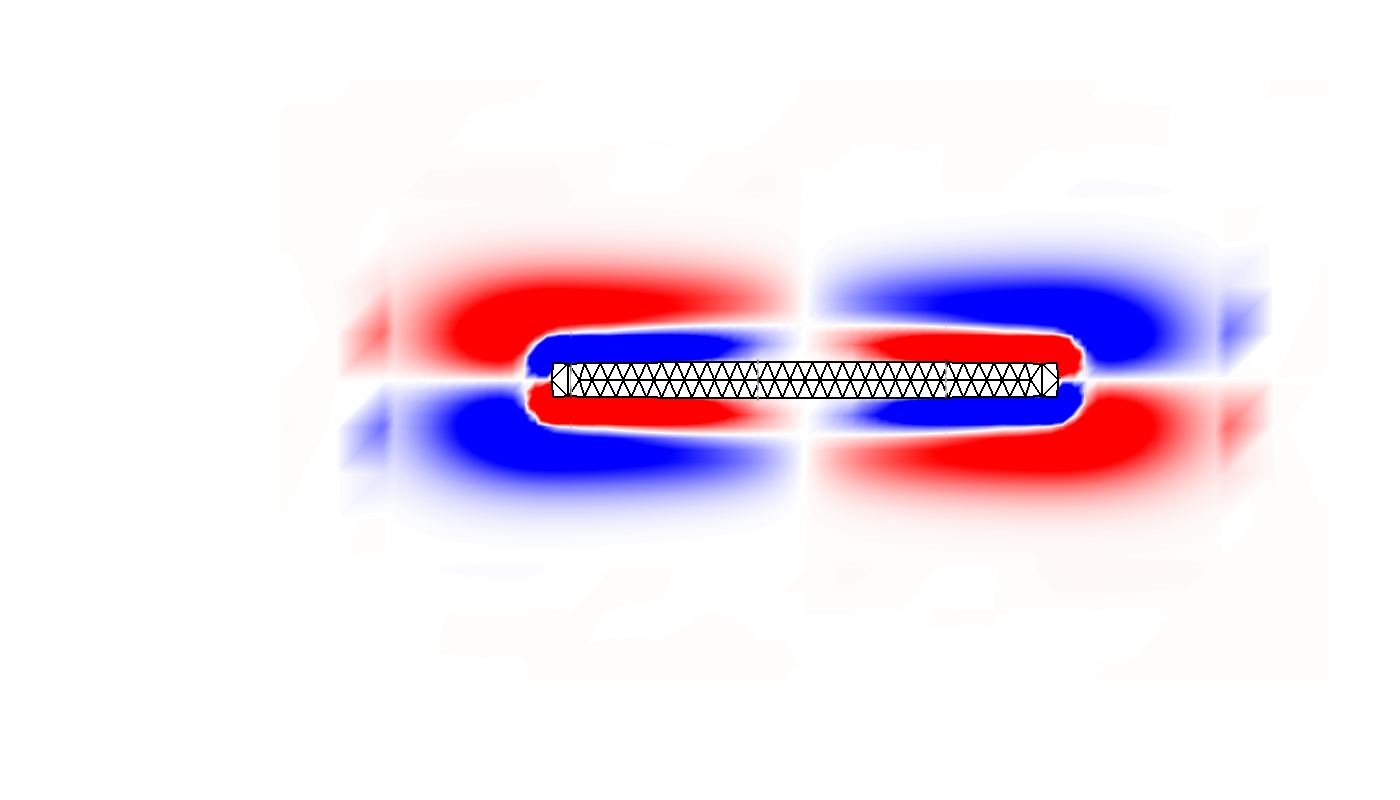
\includegraphics[width=0.8\textwidth]{ch20-static-t02.png}\\ \scriptsize $t = 0.2$: tension on; length $0.676$
\column{0.5\textwidth}\centering 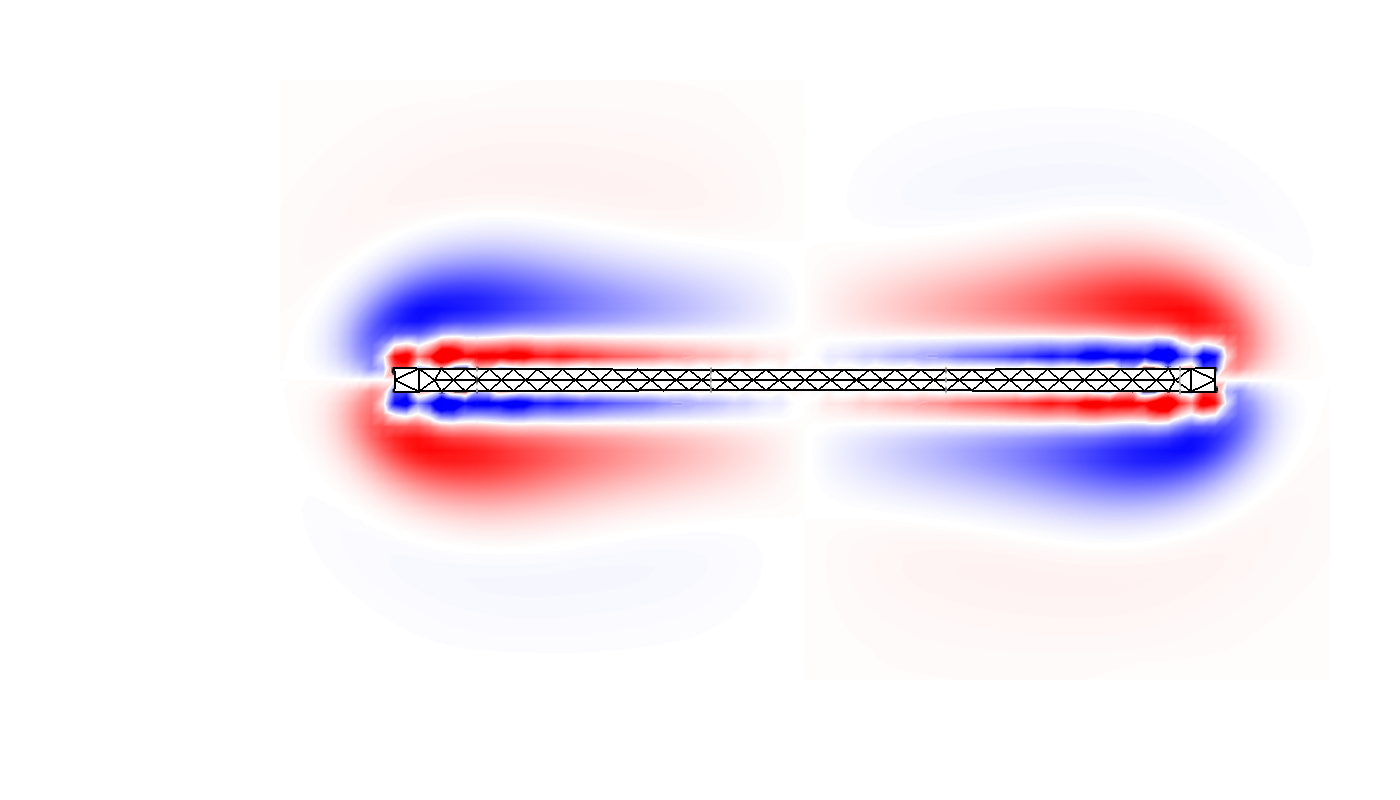
\includegraphics[width=0.8\textwidth]{ch20-static-t08.png}\\ \scriptsize $t = 0.8$: tension off since $0.5$; length $1.094$
\end{columns}
\scriptsize
\begin{tabular}{@{}llL{0.60\textwidth}@{}}
\toprule
time & length & notes \\
\midrule
$0$ & $1.000$ & \\
$0.2$ & $0.676$ & shortest in the first cycle; the plate is $0.047$ thick instead of $0.031$ (volume kept) \\
$0.4$ & $0.786$ & still under tension, but slightly longer again \\
$0.8$ & $1.094$ & tension off since $t = 0.5$: the plate overshoots its rest length \\
$1.2$ & $0.663$ & the next cycles repeat this ($0.663$ at $t = 2.2$, $0.662$ at $3.2$) \\
\bottomrule
\end{tabular}

\sourcecredit{Length: distance between the nodes that start at $x = \pm0.5$ on the centre line, from \code{output.ex2}. Window $[-0.7, 0.7]\times[-0.4, 0.4]$, vorticity $\pm5$.}
\end{frame}

% 11
\begin{frame}{STATIC (2): the fourth cycle, and what the numbers say}
\label{fr:static2}
\begin{columns}[T]
\column{0.42\textwidth}
\begin{center}
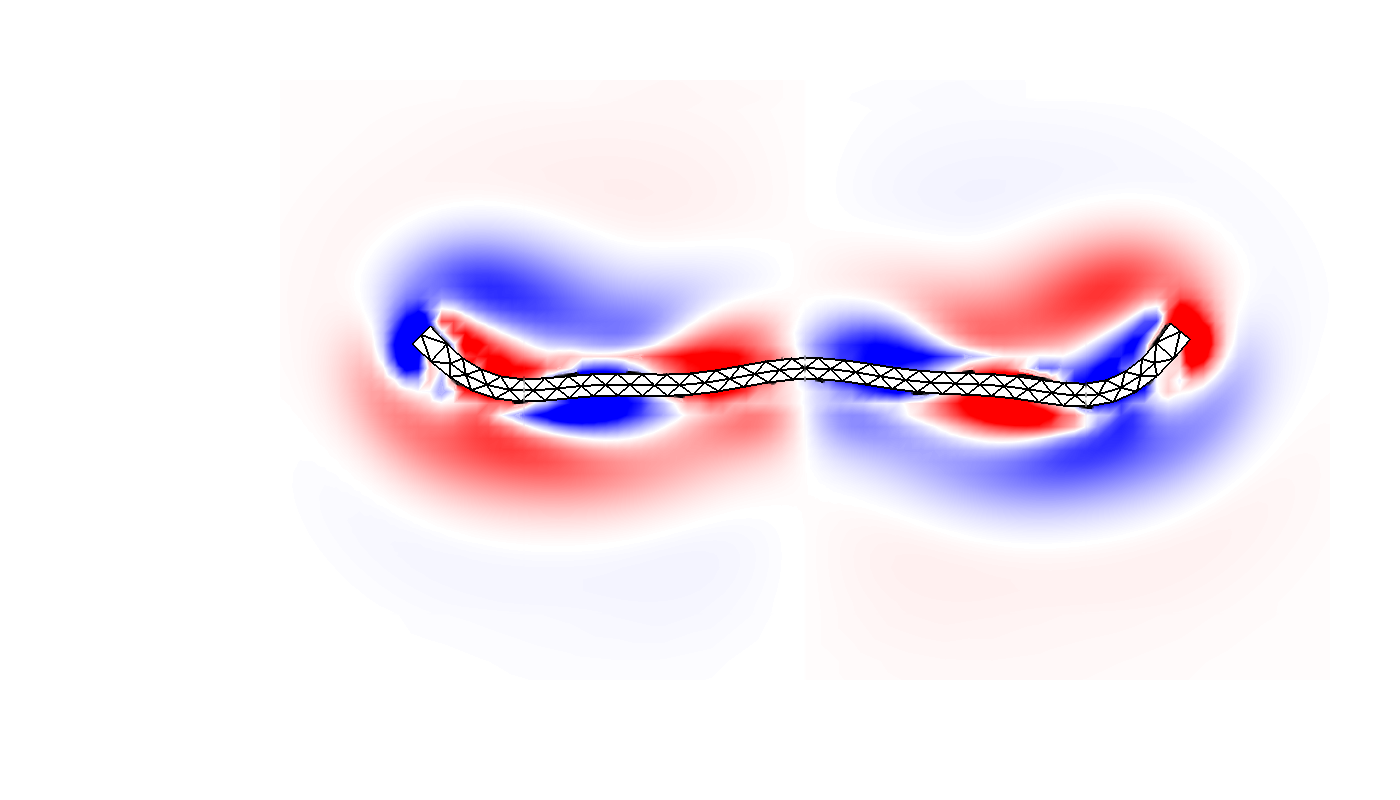
\includegraphics[width=\textwidth]{ch20-static-t38.png}\\ \scriptsize $t = 3.8$: the middle $0.047$ below the ends
\end{center}
\column{0.56\textwidth}
\footnotesize
\begin{itemize}
  \item With $T = 20$ against $\mu = 10$ the plate shortens by a third and thickens to keep its area: the fluid's incompressibility at work (chapter 19, slide 7).
  \item The shortening takes $0.2$ s and the plate is already lengthening again at $0.4$ while the tension is still on: the fluid it pushed out of the way comes back and the elastic recoil fights the muscle. The overshoot to $1.094$ after release is the same inertia and elasticity the other way.
  \item In the fourth cycle the plate starts to bend: a straight plate under axial compression is unstable, and the bend grows from tiny asymmetries. This part of the run is the most sensitive to round-off (0.16.0 and 0.19.0 differ there by $10^{-5}$). A real muscle strip would do the same.
  \item The true tension at the shortest length is $T\lambda^2 \approx 20\times0.68^2 = 9$ (slide \ref{fr:formula}); the passive stress that balances it is $\mu(\lambda - 1/\lambda) \approx 10\times(0.68 - 1.47) = -7.9$ per reference length, so most of the contraction is set by $T$ against $\mu$ and the rest by the fluid's drag.
\end{itemize}
\end{columns}
\end{frame}

% 12
\begin{frame}{MOVING: a travelling pulse, and a plate that swims}
\label{fr:moving}
\begin{columns}[T]
\column{0.5\textwidth}\centering 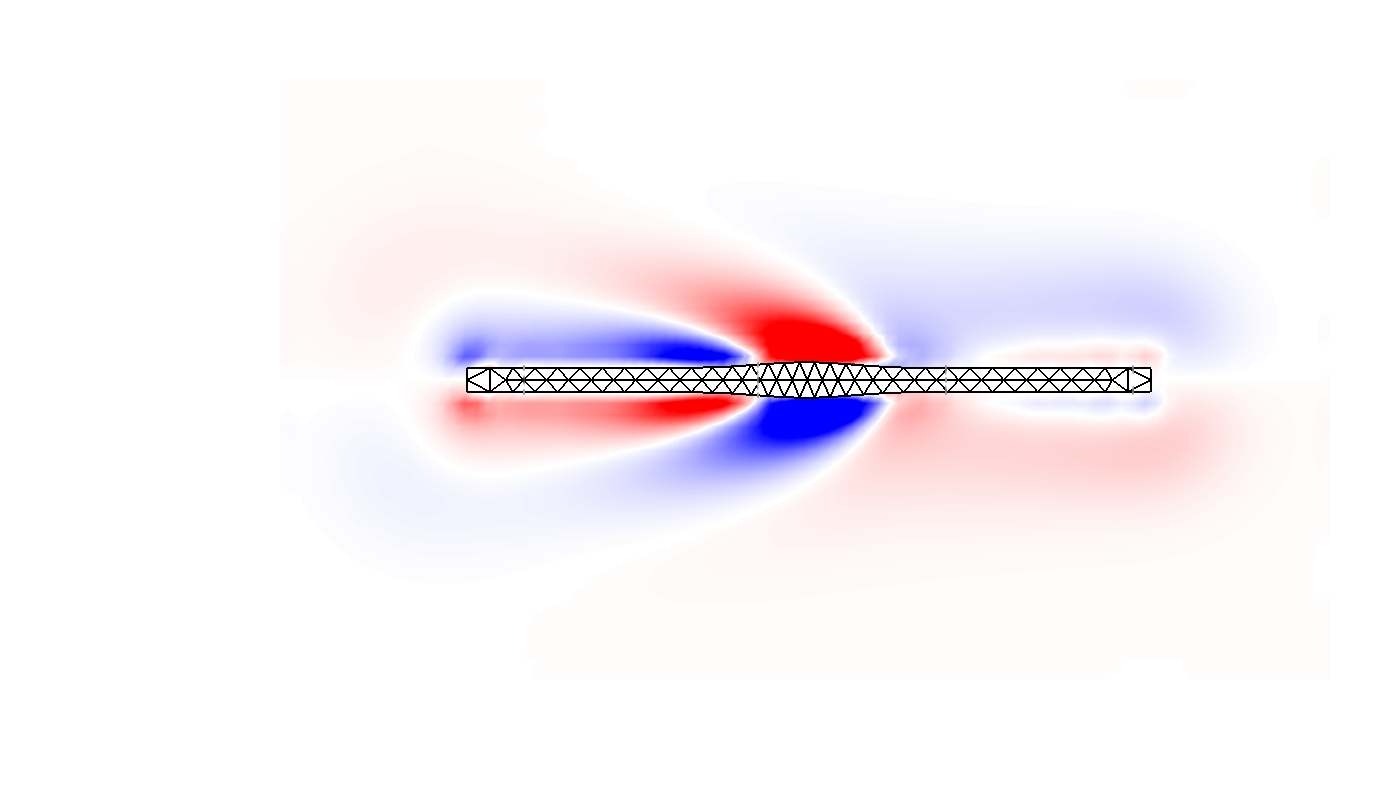
\includegraphics[width=0.8\textwidth]{ch20-moving-t05.png}\\ \scriptsize $t = 0.5$: the pulse at the plate's centre
\column{0.5\textwidth}\centering 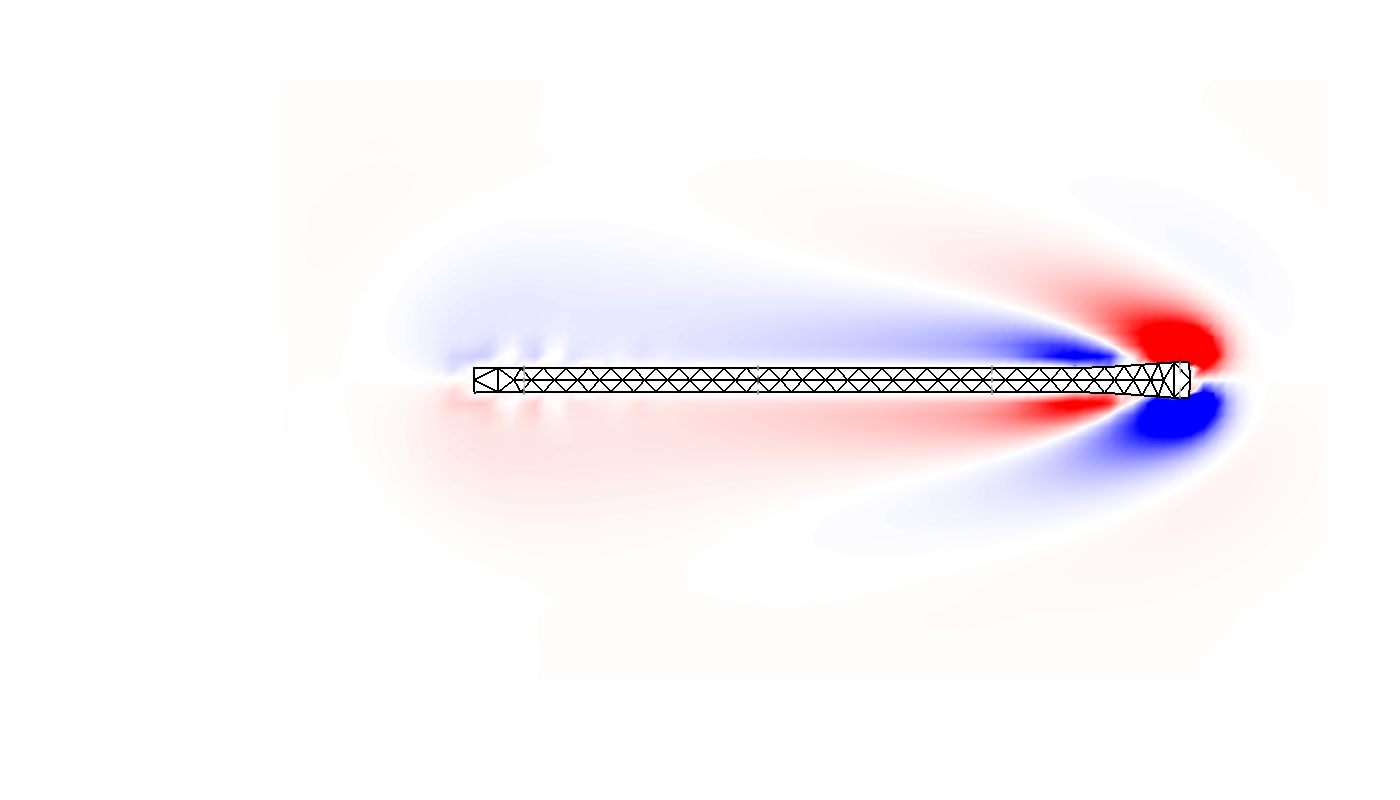
\includegraphics[width=0.8\textwidth]{ch20-moving-t40.png}\\ \scriptsize $t = 4$: four pulses later, the plate has moved right
\end{columns}
\scriptsize
\begin{itemize}
  \item A Gaussian pulse of tension, width $0.1$ (three elements), peak $40$, travels from the left end to the right end once a second. The plate stays straight; its length stays between $0.910$ and $0.961$ as the pulse passes.
  \item It swims slowly \emph{in the direction the pulse travels}: its centre is at $x = 0.014$ at $t = 1$, $0.027$ at $2$, $0.041$ at $3$ and $0.054$ at $4$: $0.0135$ per cycle, steadily. A local contraction moving along a body in a viscous fluid is a peristaltic swimmer; the asymmetry between the material that contracts ahead of the pulse and relaxes behind it is what pushes the fluid backwards.
  \item ``The applied tension translates along the length causing a local region of contraction'' (2014): the figure at $t = 0.5$ shows the contracted region as the thickened middle and the pair of vortices it drives.
\end{itemize}
\sourcecredit{IBFE/06, \code{FIBER\_MODE = "MOVING"}, IBAMR 0.19.0; \code{wsl/final/visit\_ch20.sh}.}
\end{frame}

% 13
\begin{frame}{ALTERNATING: one side only, and the plate bends}
\label{fr:alternating}
\begin{columns}[T]
\column{0.5\textwidth}\centering 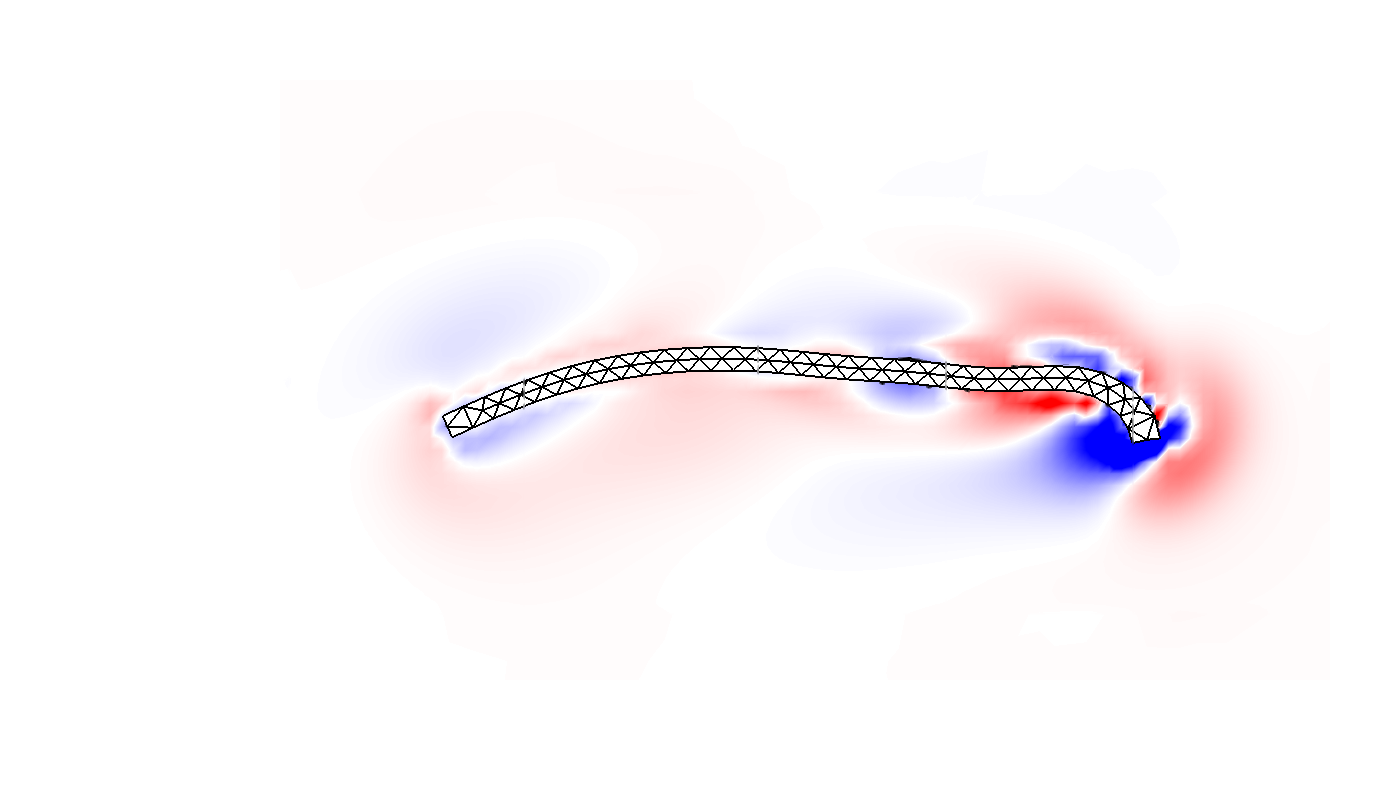
\includegraphics[width=0.8\textwidth]{ch20-alt-t20.png}\\ \scriptsize $t = 2$: bend $0.091$
\column{0.5\textwidth}\centering 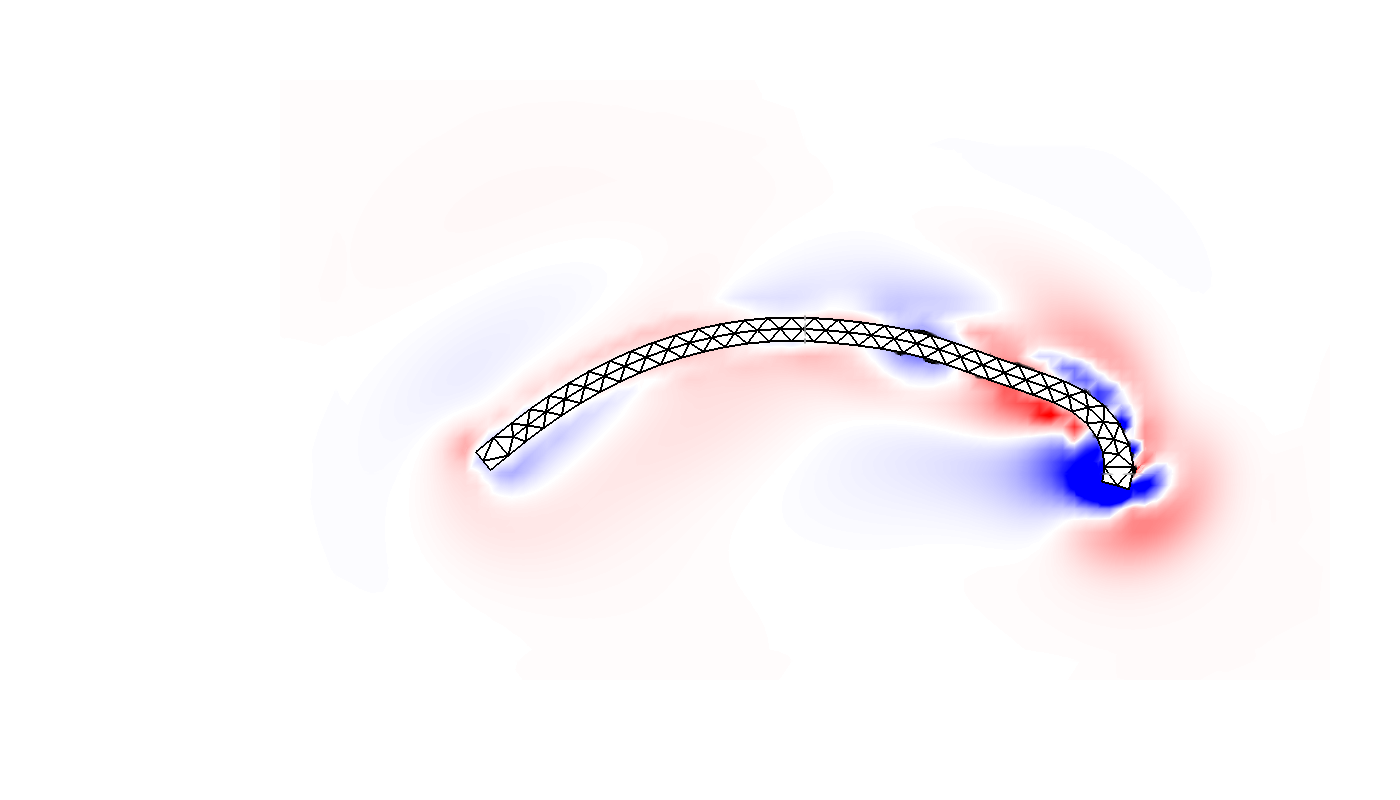
\includegraphics[width=0.8\textwidth]{ch20-alt-t40.png}\\ \scriptsize $t = 4$: bend $0.191$
\end{columns}
\scriptsize
\begin{itemize}
  \item The same pulse (peak $30$) in the bottom half of the plate only: the bottom shortens, the top does not, so the plate bends with its ends down. The bend (height of the middle node above the mean of the ends) grows every cycle: $0.038$ at $t = 1$, $0.091$ at $2$, $0.148$ at $3$, $0.191$ at $4$.
  \item This is the simplest model of a bending muscle: contraction on one side of a neutral line. A body that alternates sides (the 2014 oscillating-muscle code, the homework's second part) undulates instead of curling.
  \item The plate is two elements thick; ``bottom half'' is the lower row of triangles (\code{s(1) < 0}, with $s(1) = \pm0.0156$ or $0$ for the three node rows). A thicker plate would resolve the bending moment better; chapter 18's ``two elements across the thickness'' is the minimum, and this is it.
\end{itemize}
\sourcecredit{IBFE/06, \code{FIBER\_MODE = "ALTERNATING"}, IBAMR 0.19.0.}
\end{frame}

% 14
\begin{frame}{$T$ against $\mu$: the stiffer plate}
\label{fr:mu40}
\begin{columns}[T]
\column{0.42\textwidth}
\begin{center}
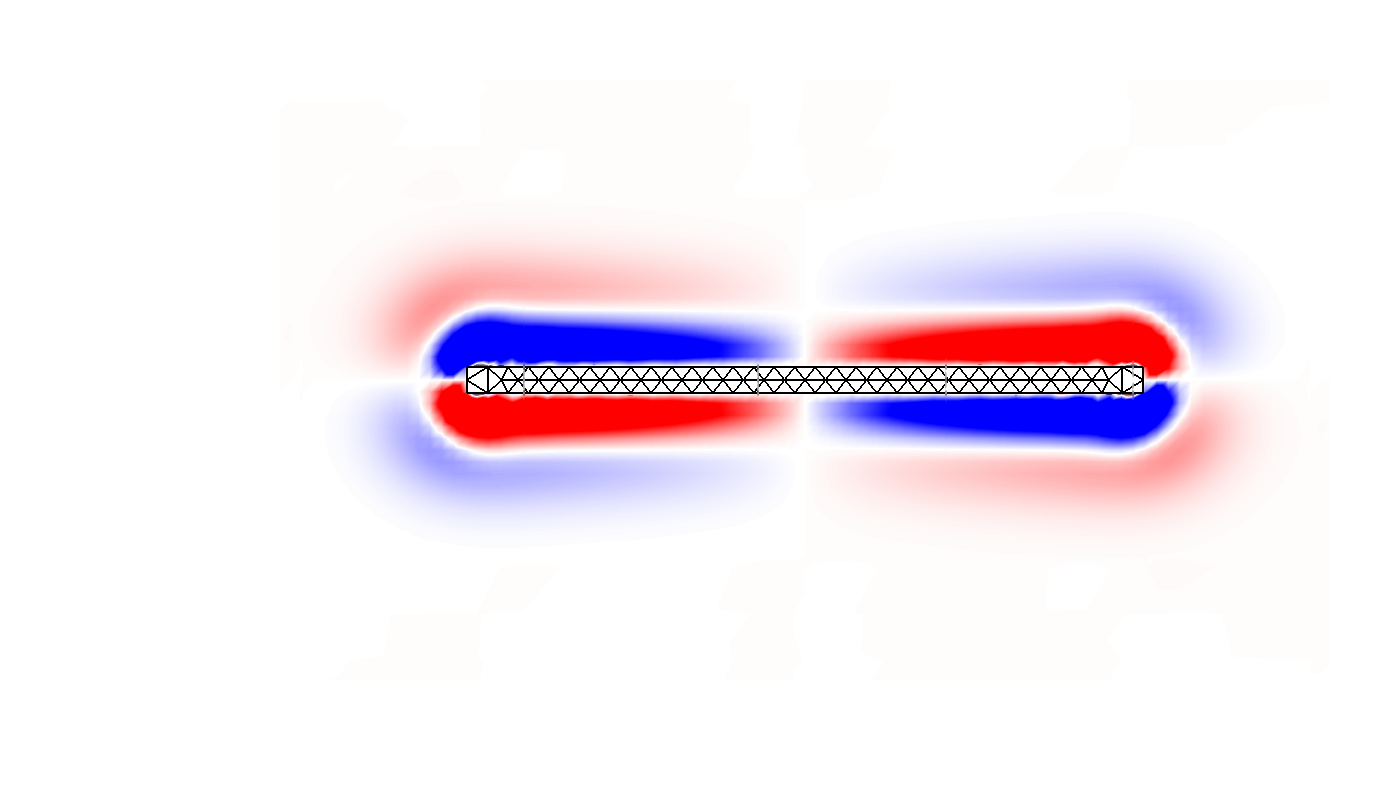
\includegraphics[width=\textwidth]{ch20-static-mu40-t02.png}\\ \scriptsize $\mu = 40$, $t = 0.2$: length $0.873$
\end{center}
\column{0.56\textwidth}
\footnotesize
\begin{itemize}
  \item \code{SHEAR\_MODULUS = 40} with the same $T = 20$: the plate shortens only to $0.873$ (instead of $0.662$) and springs back to at most $1.033$ (instead of $1.094$).
  \item The balance $T\lambda^2 \approx \mu(1/\lambda - \lambda)$ gives $\lambda \approx 0.69$ for $T/\mu = 2$ and $0.87$ for $T/\mu = 0.5$: close to the measured $0.68$ and $0.87$, so the static shortening is set almost entirely by the ratio $T/\mu$, the fluid's drag mattering only for how fast.
  \item So the non-dimensional number to report with a muscle model is $T_{\max}/\mu$ (and the convention, slide \ref{fr:formula}), together with the time scale of the activation against the body's elastic response time $\sqrt{\rho L^2/\mu}$ ($0.32$ here against the $0.5$ s contraction).
  \item The same $T$ on a stiffer plate is a weaker muscle in effect; to keep the motion when you change $\mu$, scale $T$ with it.
\end{itemize}
\end{columns}
\sourcecredit{Run: \code{/root/work/0.19.0/ibfe06\_STATIC\_mu40}, IBAMR 0.19.0 (the README's ``Things to try'').}
\end{frame}

% 15
\begin{frame}[fragile]{The homework, and the tension that must not go negative}
\label{fr:homework}
\footnotesize
``Take example 2 and apply tension as a sine wave that travels down the body. Note that you want to use something like \code{1.0/2.0* (1.0+sin((2.0*pi*(s(0)/body\_length + time)))} to not create negative tension. Squeeze the top and the bottom out of phase using the traveling sine wave (see example 3 for ideas)'' (2014, slide 11; 2020, slide 23).
\begin{itemize}
  \item The slide's expression has one more \code{(} than \code{)}; the intended tension is
  \[ T(\mathbf{s}, t) = \tfrac12\,T_{\max}\bigl(1 + \sin 2\pi(s_0/L + t)\bigr), \]
  a wave of wavelength $L$ (the plate's length) travelling in the $-x$ direction at speed $L$ per unit time, with $0 \le T \le T_{\max}$.
  \item Why the $\tfrac12(1 + \sin)$: a plain $T_{\max}\sin(\cdot)$ is negative half the time, and a negative $T$ pushes along the fibres: the slender plate buckles and the run stops. Muscle only pulls; the offset keeps the model honest.
  \item In IBFE/06, replace the two lines after the \code{if} of the \code{MOVING} case by
\end{itemize}
\begin{lstlisting}[style=cpptiny]
const double body_length = 1.0;
return 0.5 * T_max * (1.0 + std::sin(2.0 * libMesh::pi * (s(0) / body_length + time)));
\end{lstlisting}
\begin{itemize}
  \item The direction the wave travels: $s_0/L + t$ constant means $s_0$ decreases as $t$ grows, so the wave moves toward $-x$; \code{s(0)/body\_length - time} sends it the other way. The 2014 Gaussian pulse moved toward $+x$.
\end{itemize}
\end{frame}

% 16
\begin{frame}[fragile]{The two solution folders (2017), and the phase that is not $180^\circ$}
\label{fr:homework2}
\scriptsize
\code{Example\_IBFE\_MovingSinusoidalFiberStress2D\_2016-11} (2017-03-22; shipped with its output):
\begin{lstlisting}[style=cpptiny]
double body_length = 1.0;	// beam length
// T is the magnitude of tension. Varies in space and time. 40 is the maximum.
double T = (40.0 /2.0) * (1.0+sin(2.0*pi*((s(0)/body_length)+time)));
\end{lstlisting}
\code{Example\_IBFE\_MovingAltSinusoidalFiberStress2D\_2016-11}:
\begin{lstlisting}[style=cpptiny]
double T = 0.0;
if (s(1) < 0) {
	T = (40.0 /2.0) * (1.0+sin(2.0*pi*((s(0)/body_length)+time+pi/2.0)));   // bottom half: shifted
}
else {
	T = (40.0 /2.0) * (1.0+sin(2.0*pi*((s(0)/body_length)+time)));          // top half
}
\end{lstlisting}
\begin{itemize}
  \item The first is the slide's formula with the parentheses closed, $T_{\max} = 40$ and \code{pi} from libMesh.
  \item The second shifts the bottom half's wave by adding \code{pi/2.0} \emph{inside} the $2\pi(\cdot)$: a phase shift of $2\pi\cdot\pi/2 = \pi^2 \approx 9.87$ rad, which is $206^\circ$ modulo $360^\circ$, not the $180^\circ$ that ``out of phase'' means. For a half-period shift, add $\tfrac12$ inside the argument (\code{+ time + 0.5}) or $\pi$ outside it (\code{sin(2.0*pi*(...) + pi)}). The $206^\circ$ version works (the folder's output shows the plate undulating), but it is $26^\circ$ off what it was meant to be.
  \item Both solutions keep \code{t\_cycle} computed and unused, the old signature, and \code{f\_0 = (-1, 0)}; both compile against 2016-11 and need chapter 17's four changes for today's IBAMR.
\end{itemize}
\end{frame}

% 17
\begin{frame}[fragile]{The 2014 oscillating-muscle example: two conventions in one function}
\label{fr:oscillating}
\scriptsize
\code{OscillatingMuscleFiber2D} (2014, generation 1 only; never ported to 2016-11): the right part of the plate ($s_0 > 0.25$) contracts in its top half during the first half-second and in its bottom half during the second, $T = 20$:
\begin{lstlisting}[style=cpptiny]
if((time-floor(time))<0.5)
  {
    if (s(1)>0.0 && s(0)>.25)
      {
        TensorValue<double> f_0(1,0);                   // (sic) a tensor with f_0 in its first row
        double J = FF.det();
        TensorValue<double> F_f = FF*f_0;
        PP = J/F_f.size()*T*FF*f_0*f_0.transpose();     // divides by |F f_0|: the unit-fibre convention, one power short
      }
    else { PP.zero(); }
  }
else
  {
    if (s(1)<0.0 && s(0)>.25)
      {
        TensorValue<double> f_0(1,0);
        double J = FF.det();
        TensorValue<double> f_prod_f;
        outer_product(f_prod_f,f_0,f_0);
        PP = J*T*FF*f_prod_f;                           // the mapped-fibre convention of the other examples
      }
    else { PP.zero(); }
  }
\end{lstlisting}
\end{frame}

% 17b
\begin{frame}{The 2014 oscillating-muscle example (2): what the two branches do}
\label{fr:oscillating2}
\footnotesize
\begin{itemize}
  \item The top half uses $\mathbb{P}_a = J\,T\,\mathbb{F}\,\mathbf{f}_0\mathbf{f}_0^T/|\mathbb{F}\mathbf{f}_0|$ (one power of $\lambda$ removed: Cauchy tension $T\lambda$), the bottom half $J\,T\,\mathbb{F}\,\mathbf{f}_0\otimes\mathbf{f}_0$ (Cauchy tension $T\lambda^2$). With $\lambda \approx 0.7$ the two halves pull with tensions that differ by $30$ per cent for the same $T$: the undulation it produced was lopsided. (The \code{TensorValue f\_0(1,0)} works only because libMesh fills the rest of the tensor with zeros.) The theory repository's warning on slide \ref{fr:formula} is this example.
  \item Neither convention is wrong; mixing them is. IBFE/06 uses the mapped one throughout; exercise 3 (slide \ref{fr:exercises}) rebuilds this example consistently.
\end{itemize}
\end{frame}

% 18
\begin{frame}[fragile]{Fibres that change direction: $\mathbf{f}_0(\mathbf{s})$}
\label{fr:fibres}
\footnotesize
The plate's fibres all run along $x$. A bell's run around it. From the oblate jellyfish template (\code{main.C}, the circumferential direction of the subumbrellar muscle):
\begin{lstlisting}[style=cpptiny]
double s_dist = sqrt(s(0)*s(0)+s(1)*s(1));                 // distance from the bell's axis (z)
VectorValue<double> f_0((-s(1)/s_dist),(s(0)/s_dist),0);   // tangent to the circle through s: a unit vector
...
outer_product(f_prod_f,f_0,f_0);
PP = J*T*FF*f_prod_f;
\end{lstlisting}
\begin{itemize}
  \item $\mathbf{f}_0(\mathbf{s}) = (-s_2/R, s_1/R, 0)$ with $R = \sqrt{s_1^2 + s_2^2}$: ``the direction is tangent to circles centered on the bell axis; $|\mathbf{f}_0| = 1$ and $\mathbf{f}_0\cdot(s_1, s_2, 0) = 0$. Positive activation produces circumferential contractile stress. At $R = 0$ the circumferential direction is undefined: avoid axis quadrature points, regularize the field, or set the activation to zero there'' (theory repository 4.3).
  \item Any direction field you can write from \code{s} goes here: along a curved beam's centre line (from its parametrization), radial, helical ($\mathbf{f}_0 = (-s_2, s_1, p)/|\cdot|$ for a pitch $p$). Normalize it: the formula assumes $|\mathbf{f}_0| = 1$, and the stress scales with $|\mathbf{f}_0|^2$ otherwise.
  \item A direction that cannot be written in closed form (from a fibre map, a DT-MRI data set, a mesh with fibre vectors per element) is stored as a system on the mesh, filled from the file after \code{initializeFEEquationSystems()}, and read in the stress function through \code{SystemData} (chapter 19, slide 22); Exodus meshes can carry it as elemental variables (chapter 18, slide 33).
\end{itemize}
\end{frame}

% 19
\begin{frame}[fragile]{The oblate jellyfish template: a pointer}
\label{fr:jellyfish}
\footnotesize
\code{IBAMR-Research-Codes/Medusa/oblate\_jellyfish\_template\_uniform/template\_uniform/} (the 2022 copy of Alex Hoover's 3D bell; a research template, allowed in the public collection; not ported to the examples yet):
\begin{tabular}{@{}L{0.22\textwidth}L{0.70\textwidth}@{}}
\toprule
\code{HexJelly\_diam4e-2.e} & the bell: a hexahedral ExodusII mesh (from Trelis), $4$ cm across, $1.5$ MB \\
\code{input3d} & water ($\mu = 10^{-3}$, $\rho = 1000$, SI), a $0.5$ m box, $4$ levels at ratio $4$ from $8$ cells ($\mathrm{DX} = 0.98$ mm), \code{MFAC = 1}, \code{T\_MAX = 200}, \code{PERIOD = 1.0}, \code{Z\_LIM}, \code{OFFSET}, \code{MU\_ELASTIC = 100}, \code{MUVAR\_ELASTIC = 400}, \code{BETA\_S = 0}, \code{ACTIVE\_QUAD\_ORDER = "SEVENTH"}, $16$ s of run \\
\code{main.C} & the circumferential $\mathbf{f}_0$ of slide \ref{fr:fibres}; the activation $T = T_{\max}\,p_b(s_3)\,\bigl(\sigma(c) - \sigma(c - \ell)\bigr)$ with $p_b$ a logistic band below \code{Z\_LIM} and the time factor a difference of two logistic ramps in the cycle phase (a smooth on--off, as the theory repository's ``smooth ramps reduce impulsive forcing''); a \code{Tension.curve} file with the maximum $T$ each step; a neo-Hookean passive law with a stiffer margin (\code{MUVAR}) \\
\code{Makefile} & the 2014-era build; a \code{CMakeLists.txt} of chapter 3's six lines replaces it \\
\bottomrule
\end{tabular}

\end{frame}

% 19b
\begin{frame}{The oblate jellyfish template (2): the paper, and the port to come}
\label{fr:jellyfish2}
\footnotesize
\begin{itemize}
  \item Reference: A. P. Hoover, B. E. Griffith and L. A. Miller, \emph{Quantifying performance in the medusan mechanospace with an actively swimming three-dimensional jellyfish model}, J.\ Fluid Mech.\ 813 (2017) 1112--1155. ``Convention and activation form as used in that paper; check against it before reusing the constants'' (theory repository).
  \item It is the 3D, biological version of IBFE/06: fibres from \code{s}, a smooth activation in space and time, $T_{\max}$ reported with the convention. Chapter 22's flow tank and chapter 27's 3D VisIt are the tools to run and look at it; a port with a CMake build, a shortened run and a README is the natural next example (IBFE/13) once this part is written.
\end{itemize}
\end{frame}

% 20
\begin{frame}{Choosing $T$, and the time step}
\label{fr:choose}
\footnotesize
\begin{itemize}
  \item \al{Against the passive stiffness:} $T_{\max}/\mu$ sets the shortening ($2 \to 0.68$, $0.5 \to 0.87$ for the plate); for a muscle that should shorten by $10$--$20$ per cent, $T_{\max}/\mu \approx 0.2$--$0.5$. Report the ratio and the convention.
  \item \al{Against the fluid:} the work the muscle does goes into elastic energy and into moving fluid; a tension that shortens the body faster than the fluid can get out of the way raises the pressure and the velocity, and the time step follows. The MOVING run's pulse at peak $40$ is a fast local contraction; its \code{DT = 1e-3} held.
  \item \al{Against the mesh:} a pulse narrower than two elements is not resolved; a step in $T$ across an element boundary is a stress discontinuity, hence the Gaussian pulse and the template's logistic ramps, and \code{SEVENTH} for the active quadrature when the profile is narrow.
  \item \al{In time:} switching $T$ on and off instantly (the STATIC mode) is an impulse; the plate's first $0.2$ s is a transient that a ramp of $0.05$ s would soften. The theory repository: ``smooth ramps reduce impulsive forcing.''
  \item \al{What to measure:} length and thickness (the strain, hence $\lambda$ and the true tension), the centre's displacement (swimming), the bend; all from \code{output.ex2} (chapter 28); the template adds the tension itself to a \code{.curve} file every step, which chapter 11's habit of writing what you will want to plot recommends.
\end{itemize}
\end{frame}

% 21
\begin{frame}{What can go wrong}
\label{fr:wrong}
\scriptsize
\begin{tabular}{@{}L{0.40\textwidth}L{0.52\textwidth}@{}}
\toprule
symptom & cause and fix \\
\midrule
the plate folds and the run stops when the tension is on & $T < 0$ somewhere (a plain sine), or $T_{\max}/\mu$ too large; use $\tfrac12(1 + \sin)$, reduce $T_{\max}$ \\
nothing happens & the active stress is not registered, or \code{T} is zero on every path (a time test that never passes: \code{time < 0.5} instead of the cycle phase) \\
\code{no matching function ... outer\_product} & \code{f\_0} declared as a \code{TensorValue} (the 2014 comment, uncommented); it is a \code{VectorValue} \\
the body shortens by half what the paper reported & the other fibre-stress convention ($T\lambda$ or $T\lambda^2$); slide \ref{fr:formula} \\
one side contracts more than the other for the same $T$ & two conventions in one function (slide \ref{fr:oscillating}); or the two halves' node rows are not what \code{s(1) < 0} selects \\
the ``out of phase'' halves are not out of phase & the shift is inside the $2\pi(\cdot)$; add $\tfrac12$ inside or $\pi$ outside (slide \ref{fr:homework2}) \\
the stress field is jagged along the body & the pulse is narrower than two elements, or a step in $T$; widen it, ramp it, raise the active quadrature order \\
\code{nan} at the bell's axis & $R = 0$ in $\mathbf{f}_0 = (-s_2, s_1)/R$; zero the activation near the axis \\
the body drifts without a pulse & a tension that does not average to zero in space leaves a net force only if the body is asymmetric: expected for the ALTERNATING plate (it curls), check \code{s(1)} if not \\
\bottomrule
\end{tabular}

\end{frame}

% 22
\begin{frame}{What the older decks had that is now Part X}
\label{fr:legacy}
\footnotesize
\begin{tabular}{@{}L{0.46\textwidth}L{0.46\textwidth}@{}}
\toprule
2014--2020 & now \\
\midrule
three folders (\code{FiberStress2D}, \code{MovingFiberStress2D}, \code{AltMovingFiberStress2D}), each with its own \code{main.C}, Makefile and a 94-core, 12-hour job script & IBFE/06 with \code{FIBER\_MODE}; four cores, under a minute \\
\code{T = 20} in the code; \code{f\_0(-1, 0)}; the \code{TensorValue f\_0} comment & \code{TENSION\_*} and \code{PULSE\_WIDTH} in the input; \code{f\_0(1, 0)} declared once as a vector \\
the seven-argument signature (2014; 2020 slide 21) & nine arguments \\
the homework formula with an unclosed parenthesis; the solutions on Drive links & the formula on slide \ref{fr:homework}; the solutions quoted on slide \ref{fr:homework2} \\
\code{OscillatingMuscleFiber2D} (2014 only, two conventions) & slide \ref{fr:oscillating}; exercise 3 \\
``Take a look at the following examples'' (three Drive links, slide 2) & the folders are in the course's 2016-11 example set; IBFE/06 is their port \\
\bottomrule
\end{tabular}

\end{frame}

% 23
\begin{frame}{Exercises}
\label{fr:exercises}
\footnotesize
\begin{enumerate}
  \item Do the homework in IBFE/06: the travelling sine wave of slide \ref{fr:homework} as a fourth mode, \code{SINE}. Measure the swimming speed over four cycles and compare it with the Gaussian pulse's $0.0135$ per cycle. Then reverse the wave's direction.
  \item The second part: shift the bottom half by exactly half a period, run, and compare the plate's shape at $t = 2$ with the 2017 solution's $206^\circ$ version (quote its formula and run it too).
  \item Rebuild the 2014 oscillating-muscle example with one convention: top half of the right part in the first half-second, bottom half in the second, mapped-fibre law in both. How does the undulation differ from the mixed version's (slide \ref{fr:oscillating})?
  \item Ramp the STATIC tension on and off over $0.05$ s (a cosine ramp on \code{t\_cycle}). How much smaller is the first transient's peak fluid speed?
  \item Vary $T_{\max}/\mu$ over $0.25$, $0.5$, $1$, $2$, $4$ at fixed $\mu = 10$ and tabulate the shortest length; compare with $T\lambda^2 = \mu(1/\lambda - \lambda)$.
  \item Change the convention to the unit-fibre law ($\mathbb{P}_a = J\widehat{T}\lambda^{-2}\mathbb{F}\mathbf{f}_0\otimes\mathbf{f}_0$) and find the $\widehat{T}$ that gives the same shortest length as $T = 20$.
  \item Give the plate helical fibres, $\mathbf{f}_0 = (\cos\theta, \sin\theta)$ with $\theta = 30^\circ$, and run STATIC. Which way does it move, and why?
\end{enumerate}
\end{frame}

% 24
\begin{frame}{Rules of thumb}
\label{fr:thumb}
\small
\begin{itemize}
  \item Active stress is a third registered \code{PK1StressFcnData}: $\mathbb{P}_a = J\,T\,\mathbb{F}\,\mathbf{f}_0\otimes\mathbf{f}_0$, $|\mathbf{f}_0| = 1$, $T \ge 0$.
  \item $T$ is a reference tension; the true one is $T\lambda^2$. Report $T_{\max}$, the profile and the convention together.
  \item $T_{\max}/\mu$ sets the shortening; $\tfrac12(1 + \sin)$ keeps a wave non-negative; a shift of half a period is $+\tfrac12$ inside the $2\pi(\cdot)$.
  \item Smooth profiles in space (two elements or wider) and time (ramps); a higher active quadrature order for narrow pulses.
  \item A pulse that travels makes the body swim the way the pulse goes; a pulse on one side makes it curl; alternating sides make it undulate.
  \item Fibre directions from \code{s} in closed form, or from a system on the mesh through \code{SystemData}; zero the activation where the direction is undefined.
  \item One convention per program.
\end{itemize}
\end{frame}

% 25
\begin{frame}{Summary}
\label{fr:summary}
\footnotesize
\begin{enumerate}
  \item A muscle is an active first Piola--Kirchhoff stress along a reference fibre direction, added to the passive law and registered as one more stress function. Its tension $T$ lives in the reference configuration; the Cauchy tension is $T\lambda^2$ in the mapped-fibre convention the course and the jellyfish model use.
  \item The course's three examples are IBFE/06's modes: a plate that shortens by a third and overshoots (STATIC), swims $0.0135$ per cycle after a travelling pulse (MOVING), and curls when the pulse runs along one side (ALTERNATING); a stiffer plate shortens less, in the ratio $T/\mu$ predicts.
  \item The homework's travelling sine wave needs the $\tfrac12(1 + \sin)$ offset; its 2017 solutions are quoted, including the phase shift that landed at $206^\circ$. The 2014 oscillating-muscle code mixed two conventions in one function.
  \item Fibre directions can be any function of the reference position, the bell's circumferential field being the standard one; the oblate jellyfish template in the research collection is the 3D case, with its activation band and ramps, and the next example to port.
\end{enumerate}
\begin{homebox}
\footnotesize Chapter 21 puts two or more meshes in one program (the two-coral target-point example, the beam that hits a circle); chapter 22 takes IBFE into 3D with the flow tank.
\end{homebox}
\end{frame}

% 27
\begin{frame}{References and credits}
\label{fr:refs}
\scriptsize
\begin{itemize}
  \item A. P. Hoover, B. E. Griffith and L. A. Miller, \emph{Quantifying performance in the medusan mechanospace with an actively swimming three-dimensional jellyfish model}, Journal of Fluid Mechanics 813 (2017) 1112--1155 (the active-stress convention and activation of the jellyfish template).
  \item B. E. Griffith and X. Luo, \emph{Hybrid finite difference/finite element immersed boundary method}, Int.\ J.\ Numer.\ Meth.\ Biomed.\ Eng.\ 33 (2017) e2888.
  \item The theory repository, chapter 4.3, ``Active stress and biological examples'' (passive and active stress; fiber-oriented active stress; jellyfish circumferential reference fibers; jellyfish activation field). \url{https://github.com/fairyflies9/Fluid-Dynamics-and-IBM-Theory}
  \item The examples of this series: IBFE/06 active tension (\code{main.cpp}, \code{input2d}, README with the measured lengths, bends and positions); \code{wsl/final/visit\_ch20.sh}. The course folders quoted: \code{Example\_IBFE\_FiberStress2D}, \code{MovingFiberStress2D}, \code{AltMovingFiberStress2D}, \code{MovingSinusoidalFiberStress2D}, \code{MovingAltSinusoidalFiberStress2D} (2016-11 set) and \code{OscillatingMuscleFiber2D} (2014 set).
  \item \code{IBAMR-Research-Codes/Medusa/oblate\_jellyfish\_template\_uniform} (Alex Hoover's 3D bell; the \code{Blubber} folders next to it are the same model with oral arms).
  \item Sources: Alex Hoover, \emph{4-IBFE Tutorial: Fiber Tension} (UNC, 2014, edited 2020; its six VisIt result renders, two per example, are superseded by this chapter's runs, slides \ref{fr:static}--\ref{fr:alternating}); \emph{4-IBFE Lecture: Apply Active Tension}, slides 15--23 (2020; ``adapted from Alex Hoover'').
\end{itemize}
\end{frame}

\end{document}
